\usepackage{graphicx}

\section{Miscellanea}

\subsection{Heterogeneous Aspect}

In addition to the Built-In Aspect, we are architecting a novel variant, termed as the Heterogeneous Aspect, to facilitate heterogeneous computing on the blockchain. Heterogeneous computing implies native applications cultivated based on operating systems, thus exploiting operating system resources, network requests, and an array of software utilities to construct sophisticated application logic. Presently, heterogeneous computing is primarily achieved via off-chain computations, including off-chain oracles.

This design addresses the inherent limitations of the Built-in Aspect. Operating within a virtual machine, the Built-in Aspect necessitates deterministic execution, resulting in confined resource access. On the other hand, the Heterogeneous Aspect is granted network access, enabling it to undertake demanding computational tasks. For example, running AI models, which are resource-intensive and yield non-deterministic execution results, might not be viable on virtual machines. However, these tasks are feasible within the Heterogeneous Aspect's framework.

The Heterogeneous Aspect, inherently a native application, is encapsulated within containers. This approach affords an expansion in the technological repertoire of the decentralized sphere by integrating advancements such as artificial intelligence, privacy computation, real-time computation, and decentralized storage. Heterogeneous Aspect's deployment and execution are handled within a heterogeneously architected computing network, a network that shares security in mutual accordance with the main network.

The differences between Built-in Aspects and Heterogeneous Aspects are shown in the table:

\begin{table}[htbp]
    \centering
    \begin{tabular}{|l|p{6cm}|p{6cm}|}
      \hline
      & Built-in Aspect & Heterogeneous Aspect \\
      \hline
      Consensus mechanism & Loaded and executed by main net validator nodes & Can be executed by heterogeneous computing nodes, and shares security with main net validation nodes \\
      \hline
      Execution environment & Executed in a deterministic sandbox environment & Supports interaction with external heterogeneous computing platforms and external networks \\
      \hline
      Runtime restrictions & Provides limited Runtime APIs, no IO/thread/async operation/network and other high-uncertainty operation capabilities & Native program, not limited by its execution capabilities \\
      \hline
    \end{tabular}
  \end{table}
  


\subsection{Difference Between Aspect and Off-chain Computation}

Off-chain computation refers to a model similar to Oracle, where computations occur on an off-chain consensus network. The consensus is reached off-chain on the calculated results before these are input into smart contracts for utilization.
The distinctions between Aspect and off-chain computation encompass:

\begin{itemize}
  \item \textbf{Security:} Relative to L1, the contrast between Aspect and off-chain computation parallels the differences between rollup and side-chain. While one shares security with the main network, the other assumes responsibility for its security.
  \item \textbf{Interoperability:} Both Aspect and off-chain computation exhibit interoperability with contracts on L1, similar to the interoperability seen within intra-chain contract interactions and across different chains. Aspect and contract execution occur synchronously within the same transaction, whereas off-chain computation and contracts establish a distributed transaction and are typically asynchronous.
  \item \textbf{Characteristics:} As an on-chain native program, Aspect forms part of the consensus process. It can operate within the context of the consensus execution process, such as customizing transaction data structures, validating methods, and appending additional transactions.
\end{itemize}

In conclusion, Aspect and off-chain computation can act as synergistic complements to each other, empowering both smart contracts and applications. However, due to its native extension features, Aspect possesses unique functionalities that off-chain computation cannot replicate.

\subsection{Execution Latency Analysis}

In this section, we present an analysis based on test data that yields a conclusion: integrating Aspect for supplementary computations during transaction execution can yield substantial benefits under certain conditions. For instance, increasing the transaction execution latency by 65\% for Aspect execution can result in a significant growth of 400 to 1200 times in EVM computational throughput.

\subsubsection{Benchmarking}

To rigorously appraise the execution overhead associated with Aspect, and to fine-tune the balance between the computational potentials of EVM and ArtWASM, a meticulous sequence of tests were anchored around the Fibonacci algorithm.

The experimental context was articulated as follows:

\begin{enumerate}
  \item ArtWASM's runtime, crafted in Go 1.21, employs WASMTime v11.0.0 as its pivotal execution engine.
  \item The testing was facilitated on a machine powered by a 2.2 GHz Haswell CPU.
  \item The referential smart contract was sculpted using Solidity version 0.8.20, setting it in contrast with the Aspect test code, designed in Assembly Script 0.27.5.
  \item To preserve the experiment's integrity, both Solidity and Assembly Script were devoid of optimizations, with Aspect's code strictly compiled under the -O0 flag. A thorough validation of the ensuing .wat file ensured an absence of compiler-infused enhancements.
\end{enumerate}

Three distinctive tests were designed to uncover the interplay between join point count and performance:

\begin{enumerate}
  \item The initial test, displayed in the Figure \ref{fig:image1}, constrained join point counts to 10, while sequentially increasing Fibonacci computation. This aimed at identify the point where ArtWASM's efficiency eclipses that of EVM.
  \item The next test, displayed in the Figure \ref{fig:image2}, executed 1600 Fibonacci iterations across both EVM and ArtWASM, with 100,000 times. This setup progressively augmented the count of join-points, enabling a nuanced correlation study between ArtWASM and EVM execution trajectories.
  \item The final test, displayed in the Figure \ref{fig:image3}, established 1 millisecond execution time limit, and concurrently increasing join point count. This test aimed to reveal the computational headroom that ArtWASM holds over EVM.
\end{enumerate}

\begin{figure}[htp]
  \centering
  \begin{minipage}{0.3\textwidth}
    \centering
    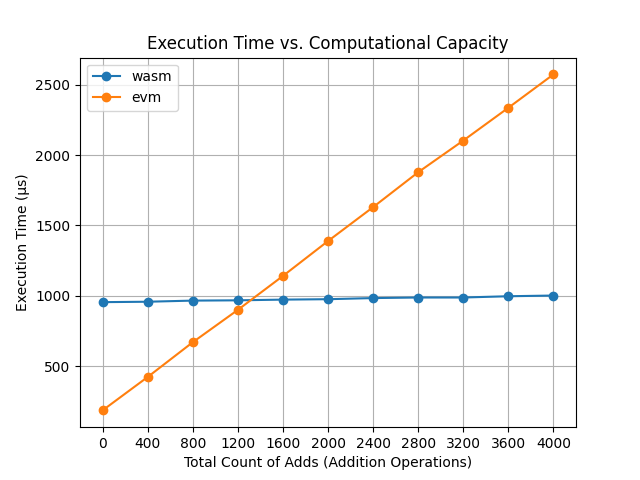
\includegraphics[width=1\linewidth]{sections/tx-latency-et-vs-cc.png}
    \caption{Equilibrium Analysis between Aspect and Smart Contract Computation}
    \label{fig:image1}
  \end{minipage}\hfill
  \begin{minipage}{0.3\textwidth}
    \centering
    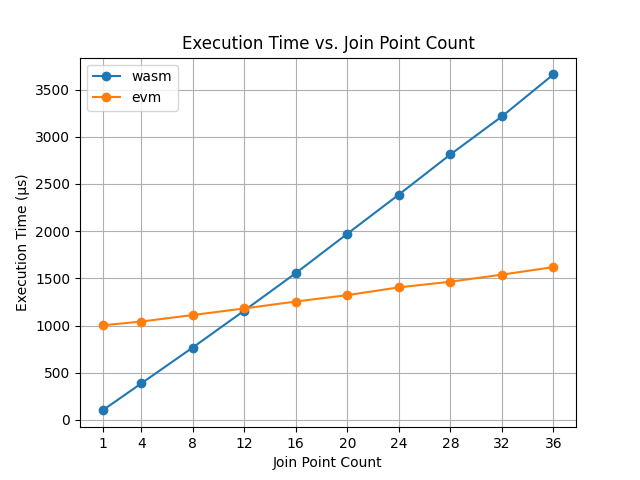
\includegraphics[width=1\linewidth]{sections/tx-latency-et-vs-jpc.png}
    \caption{Performance Interrelation between ArtWASM and EVM}
    \label{fig:image2}
  \end{minipage}\hfill
  \begin{minipage}{0.3\textwidth}
    \centering
    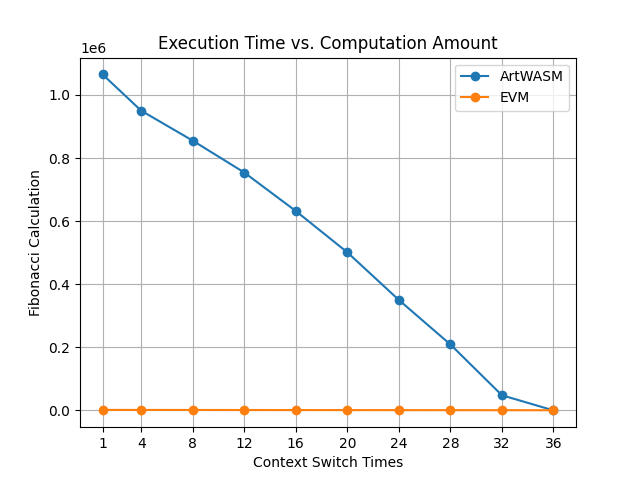
\includegraphics[width=1\linewidth]{sections/tx-latency-na-vs-jpc.png}
    \caption{Performance Delineation of ArtWASM and EVM}
    \label{fig:image3}
  \end{minipage}
\end{figure}

From the test shown in Figure \ref{fig:image1}, it can be concluded that the context switch overhead for ArtWASM is 29.5 microseconds, whereas for EVM it is 18.8 microseconds. The context switch overhead of ArtWASM is 1.57 times that of EVM in terms of performance. However, the execution performance of ArtWASM surpasses that of EVM by a factor of 2026.

When the Fibonacci computation count is 0, the execution time is equal to the context switch time. Hence, the average context switch overhead for both ArtWASM and EVM can be determined. As the computation count increases, the incremental increase in execution time for EVM far exceeds that of ArtWASM. After subtracting the context switch overhead, the execution time of EVM is 2026 times that of ArtWASM.

From the test shown in Figure \ref{fig:image2}, we can observe that when context switch time is 32, the execution time is about the same as a single EVM call. Which means if we modularize the dApp and migrate the logics from smart contract to Aspect, it is recommanded that the number of join-points used to be less than 32.

The last test shown in Figure \ref{fig:image3} emphasizes that, when the execution time is fixed, the higher the number of join points, the greater the proportion of context switch overhead, and the less time available for actual computation. When the number of join points reaches 33, there will be no time left for execution.

\subsubsection{conclusions}
The gleaned insights coalesce into several pivotal conclusions:

\begin{enumerate}
  \item Contextual switches between join-points induce a bit more overhead than an EVM call.
  \item ArtWASM's computational prowess markedly overshadows that of the EVM.
  \item It's economically prudent to nestle intricate logic within Aspect, relegating simpler logic to the smart contract.
  \item Pruning the number of join-points harnessed yields cost efficiencies.
\end{enumerate}

Distilling the insights, we can encapsulate the dynamics in the equation:

\[
  \text{ExtraComputationCapacity} \equiv \frac{\text{AspectExecTime} - \text{ContextSwitchLatency} \times \text{JoinPointNumber}}{\text{EVMExecutionLatency} \times \frac{1}{2026}}
\]

It is recommanded to adjust the Aspect execution latency dynamically for the given blockchain platform. For example, in harmony with prevailing usage patterns, we postulate:

\begin{enumerate}
  \item Aspect aims to accommodate transaction execution latencies with a moderate 65\% uptick.
  \item Of this latency, 45\% is earmarked for context switching.
  \item The residual 20\% is allocated for execution.
\end{enumerate}

Leveraging the aforementioned postulates and empirical findings, and with Ethereum's average transaction latency as our baseline, our assumptions suggest that up to 15 join-points can be executed per transaction, heralding a monumental 40000\% surge in execution performance for the system. This is just a theoretical assumption specifically for Artela, and the actual number of join-points should be adjusted according to the actual blockchain platform.
